\begin{center}
	ĐỀ ÔN TẬP KIỂM TRA GIỮA HỌC KỲ I – MÔN VẬT LÝ 11\\
	Thời gian làm bài: 50 phút \\
	(Không kể thời gian phát đề)\\
\end{center}
\ANSMCQ{
	\begin{center}
		\begin{tabular}{|m{2.8em}|m{2.8em}|m{2.8em}|m{2.8em}|m{2.8em}|m{2.8em}|m{2.8em}|m{2.8em}|m{2.8em}|m{2.8em}|}
			\hline
			1D & 2D & 3B & 4A & 5D & 6C & 7C & 8A & 9D & 10A\\
			\hline
			11D & 12A & 13D & 14C & 15D & 16B & 17C & 18B & 19B & 20B\\
			\hline
			21C & 22C & 23C & 24D & 25B & 26C & 27C & 28B & 29D & 30C\\
			\hline
		\end{tabular}
\end{center}}
\begin{enumerate}[label=\bfseries Câu \arabic*:]
	\item Một chất điểm dao động điều hòa trên trục $Ox$. Vectơ gia tốc của chất điểm có
	\begin{mcq}
		\item độ lớn cực đại ở vị trí biên, chiều luôn hướng ra biên.
		\item độ lớn cực tiểu khi qua vị trí cân bằng luôn cùng chiều với vectơ vận tốc.
		\item độ lớn không đổi, chiều luôn hướng về vị trí cân bằng.
		\item độ lớn tỉ lệ với độ lớn của li độ, chiều luôn hướng về vị trí cân bằng.
	\end{mcq}
\hideall{
\textbf{Đáp án D.}
}

\item Phát biểu nào sau đây là \textbf{sai}? Cơ năng của dao động điều hòa bằng 
\begin{mcq}
	\item động năng của vật khi đi qua vị trí cân bằng.
	\item tổng động năng và thế năng ở thời điểm bất kì.
	\item thế năng của vật ở vị trí biên.
	\item động năng ở thời điểm ban đầu.
\end{mcq}
\hideall{
\textbf{Đáp án D.}\\
Động năng ở thời điểm ban đầu không phải lúc nào cũng là động năng cực đại.
}

\item Chu kì dao động điều hòa là
\begin{mcq}
	\item khoảng thời gian để vật đi từ biên này sang biên kia.
	\item khoảng thời gian ngắn nhất để vật lặp lại trạng thái dao động.
	\item số dao động toàn phần vật thực hiện được trong $\SI{1}{\second}$.
	\item khoảng thời gian ngắn nhất để vật trở lại vị trí ban đầu.
\end{mcq}
\hideall{
\textbf{Đáp án B.}
}

\item Phát biểu nào sau đây là \textbf{sai} khi nói về dao động tắt dần?
\begin{mcq}
	\item Tần số của dao động càng lớn thì dao động tắt dần càng nhanh.
	\item Cơ năng của dao động giảm dần.
	\item Biên độ của dao động giảm dần.
	\item Lực cản càng lớn thì sự tắt dần càng nhanh.
\end{mcq}
\hideall{
\textbf{Đáp án A.}\\
Tần số của dao động càng lớn thì năng lượng dao động càng lớn, do đó sự tắt dần diễn ra càng chậm.
}

\item Con lắc đơn gồm vật nhỏ khối lượng $m$ được nối với dây treo nhẹ, không dãn. Kích thích cho con lắc dao động điều hoà thì tần số dao động của con lắc là $f$. Nếu giảm khối lượng vật nhỏ đi 2 lần thì tần số dao động của con lắc sẽ
\begin{mcq}(4)
	\item tăng $\sqrt{2}$ lần.
	\item giảm $\sqrt{2}$ lần
	\item giảm 2 lần.
	\item không đổi.
\end{mcq}
\hideall{
\textbf{Đáp án D.}\\
Tần số dao động của con lắc đơn không phụ thuộc vào khối lượng vật nặng
$$f=\dfrac{1}{2\pi}\sqrt{\dfrac{g}{\ell}}.$$
}

\item Vật nhỏ dao động điều hoà với biên độ $A$, tốc độ của vật lớn nhất khi
\begin{mcq}(2)
	\item vật ở vị trí biên âm.	
	\item vật ở vị trí biên dương.
	\item vật ở vị trí cân bằng.	
	\item vật ở vị trí có li độ $A/3$.
\end{mcq}
\hideall{
\textbf{Đáp án C.}
}

\item Dao động duy trì là dao động tắt dần mà người ta đã
\begin{mcq}
	\item Làm mất lực cản của môi trường đối với vật chuyển động.
	\item Tác dụng vào vật một ngoại lực biến đổi điều hòa theo thời gian.
	\item Cung cấp cho vật một phần năng lượng đúng bằng năng lượng của vật bị tiêu hao trong từng chu kì.
	\item Kích thích lại dao động sau khi dao động bị tắt hẳn.
\end{mcq}
\hideall{
\textbf{Đáp án C.}
}

\item Thế năng của con lắc đơn tại vị trí có li độ dài $s$ được xác định bởi công thức
\begin{mcq}(4)
	\item $W_\text{t}=\dfrac{1}{2}mg\dfrac{s^2}{\ell}$.
	\item $W_\text{t}=\dfrac{1}{2}mg\ell s^2$.
	\item $W_\text{t}=\dfrac{1}{2}mg\dfrac{s^2}{\ell^2}$.
	\item $W_\text{t}=\dfrac{1}{2}mg\dfrac{s}{\ell}$.
\end{mcq}
\hideall{
\textbf{Đáp án A.}
}

\item Một con lắc lò xo gồm vật nhỏ và lò xo nhẹ, dao động điều hòa trên mặt phẳng nằm ngang không ma sát. Động năng của con lắc đạt giá trị cực đại khi
\begin{mcq}(2)
	\item lò xo có chiều dài cực đại.
	\item vật có tốc độ cực tiểu.
	\item vật đi qua vị trí biên âm.
	\item lò xo không biến dạng.
\end{mcq}
\hideall{
\textbf{Đáp án D.}\\
Đối với con lắc lò xo dao động trên mặt phẳng nằm ngang không ma sát thì vị trí lò xo không biến dạng trùng với vị trí cân bằng của vật nặng. Khi vật qua VTCB thì vật đạt tốc độ cực đại, do đó động năng của vật đạt cực đại.
}

\item Khi nói về năng lượng của một vật dao động điều hòa, phát biểu nào sau đây là \textbf{đúng}?
\begin{mcq}
	\item Cứ mỗi chu kì dao động của vật, có bốn thời điểm thế năng bằng động năng.
	\item Thế năng của vật đạt cực đại khi vật ở vị trí cân bằng.
	\item Động năng của vật đạt cực đại khi vật ở vị trí biên.
	\item Thế năng và động năng của vật biến thiên cùng tần số với tần số của li độ.
\end{mcq}
\hideall{
\textbf{Đáp án A.}\\
Cứ mỗi chu kì dao động của vật, có bốn thời điểm thế năng bằng động năng ứng với vị trí $x=\pm\dfrac{A}{\sqrt{2}}$.\\
Thế năng của vật đạt cực đại khi vật ở vị trí biên.\\
Động năng của vật đạt cực đại khi vật ở vị trí cân bằng.\\
Thế năng và động năng của vật biến thiên với tần số gấp 2 lần tần số của li độ.
}

\item Một vật dao động điều hòa trên trục $Ox$. Hình bên là đồ thị biểu diễn sự phụ thuộc của li độ $x$ vào thời gian $t$. Tần số của dao động là 
\begin{center}
	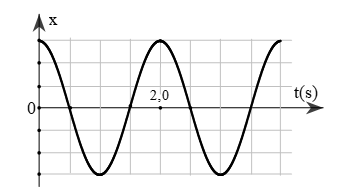
\includegraphics[width=0.4\linewidth]{../figs/D11-3-3}
\end{center}
\begin{mcq}(4)
	\item $\SI{2.0}{\hertz}$.
	\item $\SI{1.0}{\hertz}$.
	\item $\SI{1.5}{\hertz}$.
	\item $\SI{0.5}{\hertz}$.
\end{mcq}
\hideall{
\textbf{Đáp án D.}\\
Chu kì dao động của vật $T=\SI{2.0}{\second}$.\\
Tần số dao động của vật:
$$f=\dfrac{1}{T}=\SI{0.5}{\hertz}.$$
}

\item Trên hình vẽ là một hệ dao động. Khi cho con lắc M dao động, thì các con lắc (1), (2), (3), (4) cũng dao động cưỡng bức theo. Hỏi con lắc nào dao động mạnh nhất trong 4 con lắc?
\begin{center}
	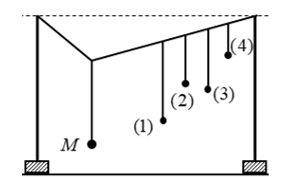
\includegraphics[width=0.4\linewidth]{../figs/D11-3-8}
\end{center}
\begin{mcq}(4)
	\item (1).
	\item (2).
	\item (3).
	\item (4)
\end{mcq}
\hideall{
\textbf{Đáp án A.}\\
Khi con lắc M dao động sẽ làm cho các con lắc còn lại dao động cường bức theo. Vì chiều dài con lắc (1) gần bằng chiều dài con lắc M nên chu kì dao động riêng của (1) xấp xỉ chu kì dao động riêng của M $\Rightarrow$ (1) dao động mạnh nhất.
}

\item Đồ thị biểu diễn li độ theo thời gian của một vật được mô tả như hình. Tốc độ của vật khi qua vị trí cân bằng là
\begin{center}
	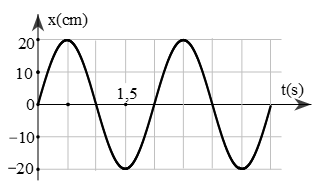
\includegraphics[width=0.4\linewidth]{../figs/D11-3-1}
\end{center}
\begin{mcq}(4)
	\item $\SI{62.8}{\meter/\second}$.
	\item $\SI{30.0}{\centi\meter/\second}$.
	\item $\SI{41.9}{\centi\meter/\second}$.
	\item $\SI{62.8}{\centi\meter/\second}$.
\end{mcq}
\hideall{
\textbf{Đáp án D.}\\
Tần số góc dao động:
$$T=\SI{2}{\second}\Rightarrow\omega=\dfrac{2\pi}{T}=\xsi{\pi}{\radian/\second}$$
Tốc độ của vật khi qua VTCB:
$$v_\text{max}=\omega A=\left(\xsi{\pi}{\radian/\second}\right)\cdot\left(\SI{20}{\centi\meter}\right)\approx\SI{62.8}{\centi\meter/\second}.$$
}

\item Một vật dao động điều hoà trên trục $Ox$. Hình bên là đồ thị biểu diễn sự phụ thuộc của li độ $x$ vào thời gian $t$. Pha ban đầu của dao động là
\begin{center}
	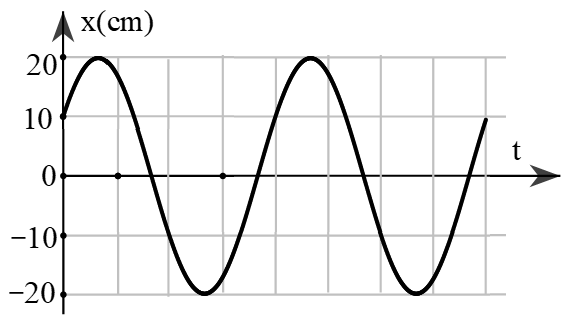
\includegraphics[width=0.4\linewidth]{../figs/D11-3-4}
\end{center}
\begin{mcq}(4)
	\item $\xsi{\dfrac{\pi}{6}}{\radian}$.
	\item $\xsi{\dfrac{\pi}{3}}{\radian}$.
	\item $-\xsi{\dfrac{\pi}{3}}{\radian}$.
	\item $-\xsi{\dfrac{\pi}{6}}{\radian}$.
\end{mcq}
\hideall{
\textbf{Đáp án C.}\\
Tại thời điểm ban đầu vật có li độ $x_0=\SI{10}{\centi\meter}$ và đang chuyển động theo chiều dương nên
$$\varphi_0=-\arccos\dfrac{x_0}{A}=-\xsi{\dfrac{\pi}{3}}{\radian}.$$
}

\item Một chất điểm dao động điều hoà có phương trình li độ $x=\xsi{6\cos\left(4\pi t-\dfrac{\pi}{3}\right)}{\centi\meter}$, thời gian $t$ tính bằng giây. Khoảng thời gian để chất điểm thực hiện được 5 dao động toàn phần là
\begin{mcq}(4)
	\item $\SI{30}{\second}$.
	\item $\SI{10}{\second}$.
	\item $\SI{2}{\second}$.
	\item $\SI{2.5}{\second}.$
\end{mcq}
\hideall{
\textbf{Đáp án D.}\\
Chu kì dao động của vật
$$T=\dfrac{2\pi}{\omega}=\SI{0.5}{\second}$$
Thời gian chất điểm thực hiện được 5 dao động là:
$$\Delta t=5T=\SI{2.5}{\second}.$$
}

\item Một vật dao động điều hoà có phương trình li độ $x=\xsi{5\cos\left(2\pi t-\dfrac{\pi}{6}\right)}{\centi\meter}$. Lấy $\pi^2=10$. Khi vật có li độ $x=\SI{3}{\centi\meter}$ gia tốc của vật là
\begin{mcq}(4)
	\item $\SI{12}{\meter/\second^2}$.
	\item $\SI{-120}{\centi\meter/\second^2}$.
	\item $\SI{1.20}{\centi\meter/\second^2}$.
	\item $\SI{12}{\centi\meter/\second^2}$.
\end{mcq}
\hideall{
\textbf{Đáp án B.}\\
Gia tốc của vật tại vị trí có li độ $x=\SI{3}{\centi\meter}$:
$$a=-\omega^2x=-\left(\xsi{2\pi}{\radian/\second}\right)^2\cdot\left(\SI{3}{\centi\meter}\right)\approx-\SI{120}{\centi\meter/\second^2}.$$
}

\item Một con lắc lò xo gồm vật năng khối lượng $\SI{400}{\gram}$ được nối với lò xo có độ cứng $\SI{100}{\newton/\meter}$. Kéo vật nặng ra khỏi vị trí cân bằng $\SI{2}{\centi\meter}$ rồi truyền cho nó tốc độ đầu $\xsi{15\sqrt{5}\pi}{\centi\meter/\second}$. Lấy $\pi^2=10$. Năng lượng dao động của vật là
\begin{mcq}(4)
	\item $\SI{245}{\joule}$.
	\item $\SI{2.45}{\joule}$.
	\item $\SI{0.245}{\joule}$.
	\item $\SI{24.5}{\joule}$.
\end{mcq}
\hideall{
\textbf{Đáp án C.}\\
Năng lượng dao động của vật là
$$W=W_\text{t}+W_\text{đ}=\dfrac{1}{2}kx^2+\dfrac{1}{2}mv^2=\SI{0.245}{\joule}.$$
}

\item Một vật dao động điều hoà với phương trình li độ $x=A\cos\left(2\pi ft+\varphi_0\right)$. Khi vật ở vị trí cân bằng thì vận tốc của vật có độ lớn
\begin{mcq}(4)
	\item $4\pi^2f^2A$.
	\item $2\pi fA$.
	\item $\pi^2f^2A$.
	\item $\pi f A$.
\end{mcq}
\hideall{
\textbf{Đáp án B.}
}
\item Một vật dao động điều hòa trong $\SI{20}{\second}$ vật thực hiện được 10 dao động toàn phần. Động năng của vật biến thiên với chu kì bằng
\begin{mcq}(4)
	\item $\SI{2.0}{\second}$.
	\item $\SI{1.0}{\second}$.
	\item $\SI{4.0}{\second}$.
	\item $\SI{0.5}{\second}$.
\end{mcq}
\hideall{
\textbf{Đáp án B.}\\
Chu kì dao động của vật:
$$T=\dfrac{\Delta t}{N}=\SI{2.0}{\second}$$
Động năng biến thiên với chu kì:
$$T'=\dfrac{T}{2}=\SI{1.0}{\second}.$$
}

\item Một vật dao động điều hoà với biên độ $A$, chu kì $T$. Thời gian ngắn nhất để vật đi từ vị trí có li độ $\dfrac{A}{2}$ đến $-\dfrac{A\sqrt{3}}{2}$ là
\begin{mcq}(4)
	\item $\dfrac{T}{8}$.
	\item $\dfrac{T}{4}$.
	\item $\dfrac{T}{6}$.
	\item $\dfrac{T}{12}$.
\end{mcq}
\hideall{
\textbf{Đáp án B.}\\
Dùng vòng tròn lượng giác hoặc trục thời gian, thời gian ngắn nhất để vật đi từ li độ $\dfrac{A}{2}$ đến li độ $-\dfrac{A\sqrt{3}}{2}$ là $\dfrac{T}{4}$.
}

\item Một vật nhỏ đang dao động điều hoà với biên độ $\SI{4}{\centi\meter}$ trên trục $Ox$, gốc toạ độ được chọn trùng với vị trí cân bằng của vật. Tại thời điểm pha của dao động là $\xsi{\dfrac{2\pi}{3}}{\radian}$ thì vật có li độ
\begin{mcq}
	\item $\SI{2}{\centi\meter}$ và chuyển động theo chiều dương trục $Ox$.
	\item $\xsi{2\sqrt{2}}{\centi\meter}$ và chuyển động theo chiều âm trục $Ox$.
	\item $\SI{-2}{\centi\meter}$ và chuyển động theo chiều âm trục $Ox$.
	\item $\SI{-2}{\centi\meter}$ và chuyển động theo chiều dương trục $Ox$.
\end{mcq}
\hideall{
\textbf{Đáp án C.}\\
Li độ của vật tại thời điểm pha dao động $\varphi=\xsi{\dfrac{2\pi}{3}}{\radian}$
$$x=A\cos\varphi=-\SI{2}{\centi\meter}$$
Vận tốc của vật
$$v=-\omega A\sin\varphi>0$$
Do đó, vật có li độ $\SI{-2}{\centi\meter}$ và chuyển động theo chiều âm trục $Ox$.
}

\item Một vật dao động điều hoà có vận tốc và li độ tại thời điểm $t_1$ và $t_2$ tương ứng là $v_1=\SI{20}{\centi\meter/\second}$, $x_1=\xsi{8\sqrt{3}}{\centi\meter}$ và $v_2=\xsi{20\sqrt{2}}{\centi\meter/\second}$, $x_2=\xsi{8\sqrt{2}}{\centi\meter}$. Vận tốc của vật có độ lớn cực đại là
\begin{mcq}(4)
	\item $\xsi{40\sqrt{2}}{\centi\meter/\second}$.
	\item $\SI{80}{\centi\meter/\second}$.
	\item $\SI{40}{\centi\meter/\second}$.
	\item $\xsi{40\sqrt{3}}{\centi\meter/\second}$.
\end{mcq}
\hideall{
\textbf{Đáp án C.}\\
Áp dụng hệ thức độc lập thời gian:
$$x^2_1+\dfrac{v^2_1}{\omega^2}=x^2_2+\dfrac{v^2_2}{\omega^2}\Rightarrow \omega=\SI{2.5}{\radian/\second}$$
Biên độ dao động của vật:
$$A=\sqrt{x^2_1+\dfrac{v^2_1}{\omega^2}}=\SI{16}{\centi\meter}$$
Vận tốc cực đại của vật:
$$v_\text{max}=\omega A=\SI{40}{\centi\meter/\second}.$$
}

\item Một chất điểm dao động điều hoà với tần số góc $\omega=\pi\approx\xsi{\sqrt{10}}{\radian/\second}$. Biết rằng khi chất điểm có vận tốc $\xsi{3\pi}{\centi\meter/\second}$ thì gia tốc của nó là $\SI{40}{\centi\meter/\second^2}$. Biên độ dao động của chất điểm bằng
\begin{mcq}(4)
	\item $\SI{3}{\centi\meter}$.
	\item $\SI{4}{\centi\meter}$.
	\item $\SI{5}{\centi\meter}$.
	\item $\SI{6}{\centi\meter}$.
\end{mcq}
\hideall{
\textbf{Đáp án C.}\\
Biên độ dao động của chất điểm
$$A=\sqrt{\dfrac{v^2}{\omega^2}+\dfrac{a^2}{\omega^2}}=\SI{5}{\centi\meter}.$$
}

\item Hình bên là hai đường hình sin biểu diễn hai trong ba đại lượng: li độ $x$, vận tốc $v$ và gia tốc $a$ theo thời gian $t$. Đường số (1) và đường số (2) lần lượt biểu diễn cho
\begin{center}
	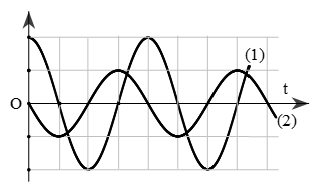
\includegraphics[width=0.4\linewidth]{../figs/D11-3-2}
\end{center}
\begin{mcq}(2)
	\item  gia tốc và vận tốc.
	\item gia tốc và li độ.
	\item vận tốc và li độ.
	\item li độ và vận tốc.
\end{mcq}
\hideall{
\textbf{Đáp án D.}\\
Nhận thấy đồ thị (2) sớm pha $\xsi{\dfrac{\pi}{2}}{\radian}$ so với đồ thị (1) nên (1) và (2) tương ứng chỉ có thể là li độ và vận tốc hoặc vận tốc và gia tốc.
}

\item Chất điểm dao động điều hoà với chu kì $\SI{2}{\second}$. Tại thời điểm $t_1$ chất điểm có li độ $\SI{3}{\centi\meter}$ và đang chuyển động theo chiều dương, sau đó tại thời điểm $t_2=t_1+\SI{0.5}{\second}$ chất điểm có li độ $\SI{4}{\centi\meter}$. Từ thời điểm $t_1$ đến thời điểm $t_2$ chất điểm có tốc độ trung bình là
\begin{mcq}(4)
	\item $\SI{2}{\centi\meter/\second}$.
	\item $\SI{6}{\centi\meter/\second}$.	
	\item $\SI{14}{\centi\meter/\second}$.
	\item $\SI{10}{\centi\meter/\second}$.
\end{mcq}
\hideall{
\textbf{Đáp án B.}\\
Li độ độ của chất điểm tại 2 thời điểm $t_1$ và $t_2$ lệch pha nhau $\xsi{\dfrac{\pi}{2}}{\radian}$ vì $\Delta t=t_2-t_2=\dfrac{T}{4}$.\\
Biên độ dao động của chất điểm:
$$A=\sqrt{x^2_1+x^2_2}=\SI{5}{\centi\meter}$$
Quãng đường chất điểm đi được từ thời điểm $t_1$ đến thời điểm $t_2$:
$$s=A-x_1+A-x_2=\SI{3}{\centi\meter}$$
Tốc độ trung bình của chất điểm trong khoảng thời gian trên:
$$v_\text{tb}=\dfrac{s}{\Delta t}=\dfrac{\SI{3}{\centi\meter}}{\SI{0.5}{\second}}=\SI{6}{\centi\meter/\second}.$$

}

\item Hình bên là đồ thị biểu diễn sự phụ thuộc li độ $x$ theo thời gian $t$ của một vật dao động điều hòa. Phương trình dao động của vật là 
\begin{center}
	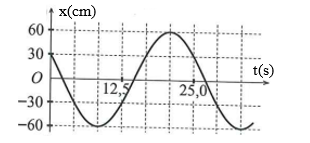
\includegraphics[width=0.4\linewidth]{../figs/D11-3-5}
\end{center}
\begin{mcq}(2)
	\item $x=\xsi{60\cos\left(\dfrac{4\pi}{45}t-\dfrac{\pi}{6}\right)}{\centi\meter}$.
	\item $x=\xsi{60\cos\left(\dfrac{4\pi}{45}t-\dfrac{\pi}{3}\right)}{\centi\meter}$.
	\item $x=\xsi{60\cos\left(\dfrac{2\pi}{25}t+\dfrac{\pi}{3}\right)}{\centi\meter}$.
	\item $x=\xsi{60\cos\left(\dfrac{4\pi}{45}t+\dfrac{\pi}{6}\right)}{\centi\meter}$.
\end{mcq}
\hideall{
\textbf{Đáp án C.}\\
Chu kì dao động của vật:
$$T=\SI{25}{\second}$$
Tần số góc dao động:
$$\omega=\dfrac{2\pi}{T}=\xsi{\dfrac{2\pi}{25}}{\radian/\second}$$
Tại thời điểm ban đầu, vật qua vị trí $x_0=\SI{30}{\centi\meter}$ theo chiều âm nên pha ban đầu
$$\varphi_0=\arccos\dfrac{x_0}{A}=\xsi{\dfrac{\pi}{3}}{\radian}$$
Phương trình dao động của vật:
$$x=\xsi{60\cos\left(\dfrac{2\pi}{25}t+\dfrac{\pi}{3}\right)}{\centi\meter}.$$
}

\item Con lắc đơn gồm vật nặng khối lượng $\SI{500}{\gram}$ được nối với sợi dây nhẹ, không dãn, đầu trên của dây được nối vào điểm cố định. Kích thích cho con lắc dao động tại nơi có gia tốc trọng trường $g=\SI{10}{\meter/\second^2}$. Lực căng của dây treo khi con lắc ở vị trí góc lệch cực đại so với phương thẳng đứng là $\SI{4}{\newton}$. Khi vật qua vị trí cân bằng thì lực căng của dây treo có độ lớn
\begin{mcq}(4)
	\item $\SI{11}{\newton}$.
	\item $\SI{5}{\newton}$.
	\item $\SI{7}{\newton}$.
	\item $\SI{3}{\newton}$.
\end{mcq}
\hideall{
\textbf{Đáp án C.}\\
Lực căng dây treo khi vật ở vị trí có góc lệch $\alpha$ so với phương thẳng đứng
$$T=mg\left(3\cos\alpha-2\cos\alpha_0\right)$$
Khi vật ở vị trí biên $\alpha=\alpha_0$
$$T_\text{biên}=mg\cos\alpha_0=\SI{4}{\newton}$$
Khi vật qua vị trí cân bằng $\alpha=\SI{0}{\radian}$:
$$T_\text{CB}=mg\left(3-2\cos\alpha_0\right)=3mg-2mg\cos\alpha_0=3\cdot\left(\SI{0.5}{\kilogram}\right)\cdot\left(\SI{10}{\meter/\second^2}\right)-2\cdot\left(\SI{4}{\newton}\right)=\SI{7}{\newton}.$$

}

\item Con lắc lò xo gồm vật nhỏ khối lượng $\SI{200}{\gram}$ nối vào đầu lò xo nhẹ, đầu còn lại của lò xo cố định vào tường. Người ta kích thích cho con lắc dao động điều hoà trên mặt phẳng nằm ngang, nhẵn. Khi vật nhỏ qua vị trí cân bằng thì nó có tốc độ $\SI{1}{\meter/\second}$. Khi vật nhỏ qua vị trí cách vị trí cân bằng đoạn $\xsi{2,5\sqrt{3}}{\centi\meter}$ thì nó có tốc độ $\SI{0.5}{\meter/\second}$. Lực đàn hồi do lò xo tác dụng lên vật nhỏ có giá trị lớn nhất là
\begin{mcq}(4)
	\item $\SI{2}{\newton}$.
	\item $\SI{4}{\newton}$.
	\item $\xsi{2\sqrt{3}}{\newton}$.
	\item $\xsi{4\sqrt{3}}{\newton}$.
\end{mcq}
\hideall{
\textbf{Đáp án B.}\\
Áp dụng hệ thức độc lập thời gian, suy ra được biên độ dao động của vật:
$$A=\dfrac{\left|x\right|}{\sqrt{1-\dfrac{v^2}{v^2_\text{max}}}}=\dfrac{\xsi{2,5\sqrt{3}}{\centi\meter}}{\sqrt{1-\left(\dfrac{\SI{0.5}{\meter/\second}}{\SI{1}{\meter/\second}}\right)^2}}=\SI{5}{\centi\meter}$$
Độ cứng của lò xo:
$$v_\text{max}=\omega A=A\sqrt{\dfrac{k}{m}}\Rightarrow k=\dfrac{v^2_\text{max}m}{A^2}=\SI{80}{\newton/\meter}$$
Lực đàn hồi cực đại của lò xo tác dụng lên vật nặng:
$$F_\text{đh max}=kA=\left(\SI{80}{\newton/\meter}\right)\cdot\left(\SI{0.05}{\meter}\right)=\SI{4}{\newton}.$$
}

\item Hai chất điểm A và B dao động điều hòa cùng tần số. Hình bên là đồ thị biểu diễn sự phụ thuộc li độ $x_1$ của chất điểm A và li độ $x_2$ của chất điểm B theo thời gian $t$. Hai chất điểm A và B lệch pha nhau
\begin{center}
	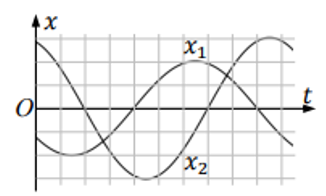
\includegraphics[width=0.35\linewidth]{../figs/D11-3-6}
\end{center}
\begin{mcq}(4)
	\item $\xsi{\dfrac{\pi}{6}}{\radian}$.
	\item $\xsi{\dfrac{\pi}{3}}{\radian}$.
	\item $\xsi{\dfrac{\pi}{12}}{\radian}$.
	\item $\xsi{\dfrac{3\pi}{5}}{\radian}$.
\end{mcq}
\hideall{
\textbf{Đáp án D.}\\
Hai vật dao động với cùng chu kì 
$$T=10\ \text{đv}$$
Sau khoảng thời gian $\Delta t=3\ \text{đv}$ thì vật 2 có cùng trạng thái dao động với vật 1 nên
$$\Delta \varphi=2\pi\cdot\dfrac{\Delta t}{T}=\xsi{\dfrac{3\pi}{5}}{\radian}.$$
}

\item Hai chất điểm A và B dao động điều hòa cùng phương, cùng tần số. Trong quá trình dao động, gia tốc của chất điểm A là $a_1$ và vận tốc của chất điểm B là $v_2$. Hình bên là đồ thị biễu diễn sự phụ thuộc của $a_1$ và $v_2$ theo thời gian $t$. Hai dao động điều hòa A và B lệch pha nhau
\begin{center}
	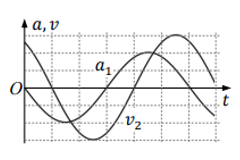
\includegraphics[width=0.35\linewidth]{../figs/D11-3-7}
\end{center}
\begin{mcq}(4)
	\item $\xsi{\dfrac{\pi}{3}}{\radian}$.
	\item $\xsi{\dfrac{5\pi}{6}}{\radian}$.
	\item $\xsi{\dfrac{\pi}{6}}{\radian}$.
	\item $\xsi{\dfrac{2\pi}{3}}{\radian}$.
\end{mcq}
\hideall{
\textbf{Đáp án C.}\\
Nhận thấy $a_1$ và $v_2$ có cùng chu kì dao động
$$T=\SI{6}{\text{đv}}$$
Sau khoảng thời gian $\Delta t=\SI{1}{\text{đv}}$ thì $v_2$ cùng pha $a_1$. Độ lệch pha $a_1$ và $v_2$:
$$\varphi_{a_1}-\varphi_{v_2}=2\pi\cdot\dfrac{\Delta t}{T}=\xsi{\dfrac{\pi}{3}}{\radian}.$$
Như vậy:
$$\varphi_{x_1}+\pi-\left(\varphi_{x_2}+\dfrac{\pi}{2}\right)=\dfrac{\pi}{3}\Rightarrow \varphi_{x_1}-\varphi_{x_2}=-\xsi{\dfrac{\pi}{6}}{\radian}
.$$
Vậy hai dao động lệch pha nhau $\Delta \varphi=\left|\varphi_{x_1}-\varphi_{x_2}\right|=\xsi{\dfrac{\pi}{6}}{\radian}$.
}
\end{enumerate}
\begin{center}
	\textbf{--- HẾT ---}
\end{center}